\nonstopmode
\documentclass[10pt, a4paper]{article}
\parindent=20pt
\parskip=8pt
\usepackage[width=15.5cm, left=3cm, top=2.5cm, height= 24.5cm]{geometry}
\usepackage[spanish]{babel}
\usepackage[utf8]{inputenc}
\usepackage{fancyhdr}
\usepackage{latexsym}
\usepackage{caratula}
\usepackage{epsfig}
\usepackage{pdfpages}
%\usepackage{algorithmicx}
\usepackage{lastpage}
\usepackage{amsfonts}
\usepackage{listings}
\usepackage{algorithm}
\usepackage{algpseudocode}
\usepackage{pdfpages}
\usepackage{amsmath}
\usepackage{verbatim}
\usepackage{graphicx}
\usepackage{float}
\graphicspath{{imgs/}}

% Acomodo fancyhdr.
\pagestyle{fancy}
\thispagestyle{fancy}
\addtolength{\headheight}{1pt}
\lhead{Teor\'ia de las Comunicaciones}
\rhead{TP3}
\cfoot{\thepage /\pageref{LastPage}}
\renewcommand{\footrulewidth}{0.4pt}
\renewcommand{\thesubsubsection}{\thesubsection.\alph{subsubsection}}


\author{Teor\'ia de las Comunicaciones, DC, UBA.}
\date{}
\title{}

\begin{document}
	
\thispagestyle{empty}
\materia{Teor\'ia de las Comunicaciones}
%\submateria{Trabajo Pr\'actico Nº1}
\titulo{Trabajo Práctico Nº3}
%\integrante{Rivero, Maximiliano}{366/07}{maxirivero088@gmail.com}
\integrante{Izcovich, Sabrina}{550/11}{sizcovich@gmail.com}
\integrante{Rogani, Marcos}{520/05}{marcos.rogani@gmail.com}

\maketitle

\tableofcontents
\newpage

\section{Introducción}
En el siguiente trabajo práctico, ejercitamos las nociones del nivel de transporte estudiadas en la materia a través de la implementación y análisis de un protocolo sencillo: \textbf{PTC}. 

El trabajo consistió, esencialmente, en simular efectos típicos de una red (tales como pérdida de paquetes o latencia) y analizar el impacto de esto en las estimaciones del RTO de un protocolo de transporte en el contexto de una red local. 

El trabajo se dividió en dos secciones: una parte implementativa y otra en la que debimos realizar experimentos, graficar resultados y extraer conclusiones sobre lo observado.

\section{Introducción Teórica}
\begin{itemize}

\item \textbf{Socket:} Un socket es en esencia un canal de comunicación entre procesos. Los sockets entre procesos remotos se llaman Internet sockets. Los sistemas operativos suelen ofrecer una interfaz para manipular sockets: conjunto de llamadas al sistema que abstraen al usuario de las problemáticas de networking que el SO resuelve, se llaman \textbf{Sockets API}.

En el contexto del tp, se utilizaron sockets raw que conforman una variante de sockets con los que los procesos pueden leer y escribir datagramas IP con un número de protocolo no procesado por el kernel del SO. Dicho campo indica qué protocolo viaja dentro de IP permitiendo diseñar e implementar protocolos de transporte ad-hoc a nivel de usuario.

\item \textbf{PTC:} Consiste en un protocolo de transporte en TCP simplificado. El mismo presenta las siguientes características:
\begin{itemize} 
\item Bidireccionalidad por ser full-duplex.
\item Orientación a conexión.
\item Confiabilidad a través de un algoritmo de ventana deslizante.
\end{itemize}

\item \textbf{RTO (Retransmission Timeout):} Consiste en la duración de un tiempo de retransmisión para asegurar el reenvío de datos en caso de ausencia de una respuesta del receptor\footnote{https://tools.ietf.org/html/rfc6298}. Para calcularlo, se utilizan dos variables de estado del sender: SRTT (smoothed round-trip time) y RTTVAR (round-trip time variation).

En primer lugar, se le asignan a dichas variables los valores que siguen:

			$$SRTT \leftarrow RTT$$
            $$RTTVAR \leftarrow RTT/2$$
            $$RTO \leftarrow SRTT + max(1, K^*RTTVAR)$$
            
con K = 4, siendo $RTT$ el primero medido.

Luego, se van actualizando siguiendo las fórmulas siguientes:

$$RTTVAR = (1 - \beta) RTTVAR + \beta |SRTT - RTT|$$
$$SRTT = (1 - \alpha)SRTT + \alpha RTT$$
$$RTO = SRTT + max(1, RTTVAR)$$

El parámetro $\alpha$ es seleccionado para regular el $SRTT$. Al elegir un $\alpha$ grande, el $RTO$ puede verse muy influenciado por una fluctuación temporaria mientras que con un $\alpha$ chico puede ser más estable pero no suficientemente rápido como para adaptarse a los cambios reales. La especificación de TCP recomienda regular a $\alpha$ entre 0.1 y 0.2.
\end{itemize}

\newpage
\section{Primera Parte: escenario de análisis}

\subsection{Experimentación variando el porcentaje de pérdida de ACK}
En primer lugar, tomando como punto de partida el código suministrado por la cátedra, implementamos ciertas modificaciones al protocolo con el fin de generar un escenario de análisis sobre el que estudiamos qué parámetros $\alpha$, $\beta$ optimizan el cálculo del RTO.

Para ello, del lado del servidor, comenzamos agregando la posibilidad de introducir un delay ($ack\_delay$) y una probabilidad $p$ de pérdida de paquetes ($ack\_loss\_probability$) al momento de enviar los ACKs. Con el fin de que fuera editable, modificamos el constructor de la clase (en el archivo $protocol.py$) para que tome el delay y la probabilidad de pérdida:
\begin{verbatim}
		def __init__(self, ack_delay=0, ack_loss_probability=0):
\end{verbatim}

Luego, modificamos la función $send\_ack$ del archivo $handler.py$ con el fin de armar el ACK para enviar una vez que llega un paquete. Para ello, agregamos lo que sigue:

\begin{verbatim}
if self.protocol.state == ESTABLISHED:
    if random.uniform(0, 1) < self.protocol.ack_loss_probability:
       print("ACKed lost segment")
       return
     if self.protocol.ack_delay > 0:
        print("Delayed ACK")
        time.sleep(self.protocol.ack_delay)
        ack_packet = self.build_packet()
        print("Sending ACK: window=%d" % ack_packet.get_window_size())
        self.socket.send(ack_packet)
\end{verbatim}
        
En el código anterior, se puede ver que el primer $if$ sirve para que se aplique el delay o pérdida únicamente si se encuentra establecida la conexión.
Luego, el condicional $if\ random.uniform(0, 1) < self.protocol.ack\_loss\_probability$ permite ver si se perdió el ACK o no, dependiendo de la probabilidad de pérdida que se le configure. En el caso en el que el paquete se pierde, realiza $return$ para terminar la función sin mandar ACK, caso contrario lo demora con $time.sleep()$, tal como se desea.

Para definir la probabilidad $p$ de pérdida de paquetes, decidimos simularla utilizando la herramienta $random.uniform(0,1)$\footnote{docs.python.org/2/library/random.html} con el fin de que la decisión de si los paquetes fueron enviados efectivamente fuera la misma que la de ``tirar una moneda'', esto es, siguiendo una distribución uniforme.

Dado que la clase que usa PTCProtocol también debe inicializarse con los parámetros mencionados anteriormente, debimos modificar la clase $Socket$ de $ptc\_socket.py$ agregando los parámetros al constructor, siendo dicha clase la que se llama para crear un nuevo Socket. Ésto se realizó de la siguiente forma:
\begin{verbatim}
class Socket(object):
    def __init__(self, ack_delay=0, ack_loss_probability=0):
		self.protocol = PTCProtocol(ack_delay=ack_delay, ack_loss_probability=ack_loss_probability)
\end{verbatim}

Por motivos que desconocemos, los cambios presentados anteriormente no generaron el resultado esperado. Testeando las modificaciones con una probabilidad de 100\% de pérdida de paquetes (es decir, perdiendo todos los ACKs de los paquetes enviados) del cliente, seguíamos recibiendo ACKs del lado del servidor. Es por esto que decidimos no enviar los paquetes del cliente directamente con cierta probabilidad en vez de simularla perdiendo sus ACKs.

\subsection{Experimentación variando el porcentaje de envío de paquetes}
Para tener la posibilidad de variar el porcentaje de paquetes enviados por el cliente, modificamos la función $send\_and\_queue$ dentro de la clase $PTCProtocol$ de la siguiente forma:
 
 \begin{verbatim}
  	if self.state == ESTABLISHED and FINFlag not in packet:
		if random.uniform(0, 1) < self.packet_loss_probability:    
			return
	self.socket.send(packet)
 \end{verbatim}
A su vez, se modificó la cadena de constructores para que el parámetro $packet\_loss\_probability$ sea configurable. A continuación, utilizamos $ack\_loss\_probability$ y $packet\_loss\_probability$ de forma indistinguida dado que las pruebas se realizaron con ambas modificaciones antes de que notáramos que los resultados eran los esperados únicamente cuando alterábamos el porcentaje de envío de paquetes. 

\newpage
\section{Segunda parte: experimentación y análisis}

En esta sección, definimos un esquema cliente-servidor en el que el cliente envía datos y el servidor se limita a reconocerlos. Para distintas combinaciones de $\alpha$ y $\beta$ debimos analizar cómo evoluciona la estimación del RTO en el cliente y buscar valores que acerquen tanto como sea posible dicha estimación al RTT ``real''. A partir de dichos resultados, analizamos cómo impactan los efectos de red simulados en los parámetros encontrados.

%%%%%%Tener en cuenta además que el protocolo mantiene la estimación en ticks, por lo que será necesario hacer la conversión a una unidad de tiempo para poder contrastarlo correctamente con el RTT.

En primer lugar, debimos realizar las modificaciones necesarias al código de forma tal que se pudieran setear los valores $\alpha$, $\beta$ y $k$. 
Para ello, modificamos el constructor de la clase $ptc\_socket$ agregándole los parámetros 
\begin{itemize}
\item alpha=0.125
\item beta=0.25
\item k=4
\end{itemize}
siendo éstos los valores por defecto en $constants.py$.

Luego, creamos una instancia del protocolo agregándole los nuevos parámetros de modo que quedara de la siguiente forma:
\begin{verbatim}
PTCProtocol(ack_delay=ack_delay, 
					ack_loss_probability=ack_loss_probability, alpha=alpha, beta=beta, k=k)
\end{verbatim}

Por otro lado, modificamos el constructor PTCProtocol para que acepte dichos parámetros de la siguiente forma:
\begin{verbatim}
def __init__(self, ack_delay=0, ack_loss_probability=0, beta, alpha, k):
\end{verbatim}

Luego, cambiamos $ALPHA$, $BETA$ y $K$ por $self.protocol.alpha$, $self.protocol.beta$ y $self.protocol.k$ respectivamente, en la función $update\_rtt\_estimation\_with$ para que dichos valores fueran los seteados desde el miembro protocolo.

Por último, creamos el servidor y el cliente de la siguiente forma:

\subsection{Server}

Para crear el servidor, se parsearon los parámetros de modo tal a moder manipular los valores convenientemente siendo éstos el \textit{delay de ACK} (con un default de 0), la \textit{probabilidad de pérdida de ACK} (con un default de 0) y el \textit{puerto} (con un default de 6677).

\begin{verbatim}
#inicializo parser
parser = argparse.ArgumentParser()
#Agrego el parametro de delay de ACK
parser.add_argument('-d', '--delay', type=float, default=0.0, help='ACK packet delay in
									 seconds (default 0)')
#Agrego el parametro de perdida de ACK
parser.add_argument('-l', '--loss', type=float, default=0.0, help='probability of losing an 
									ACK packet (default 0)')
#Agrego el parametro de puerto
parser.add_argument('-p', '--port', type=int, default=6677, help='PTC port')
args = parser.parse_args()
\end{verbatim}

En primer lugar, se liga al socket a la ipServer con el puerto ingresado como parámetro. Luego, se lo pone en estado de $listen$ a la espera de que algún cliente desee conectarse. Una vez que recibe un pedido remoto de conexión, lo acepta y devuelve un nuevo socket con la conexión establecida. Más tarde, obtiene la cantidad de bytes que va a recibir y los recibe dentro del ciclo. Una vez recibidos todos los bytes, se cierra el socket.

\begin{verbatim}
with Socket(ack_delay=args.delay, ack_loss_probability=args.loss) as sock:
    sock.bind((ipServer, args.port))
    sock.listen()
    print 'Waiting for a client...'
    sock.accept()
    print 'Connection established.'
    size = unpack('I', sock.recv(4))[0]
    print 'Receiving %d bytes...' % size
    received = str()
    #Un while que solo reciba los datos y los lea del buffer
    #Guarda los datos recibidos en received (print para verlo)
    while len(received) < size:
        received += sock.recv(size - len(received))
        print 'Received %d bytes.' % len(received)

    sock.close()
    print 'Received %d bytes. Connection closed.' % size
\end{verbatim}

\subsection{Client}
\begin{verbatim}
parser = argparse.ArgumentParser()
parser.add_argument('--host', help='Server hostname')
parser.add_argument('-p', '--port', type=int, help='Server port')
parser.add_argument('-s', '--size', type=int, help='Bytes to send')
parser.add_argument('-a', '--alpha', type=float, help='Alpha', default=0.125)
parser.add_argument('-b', '--beta', type=float, help='Beta', default=0.25)
parser.add_argument('-k', '--kvar', type=float, help='K', default=4)
args = parser.parse_args()
\end{verbatim}

En primer lugar, se parsearon los parámetros de modo tal a moder manipular los valores convenientemente siendo éstos el \textit{Server hostname}, el \textit{Puerto}, el \textit{tamaño de los bytes a enviar}, $\alpha$, $\beta$ y $k$.

\begin{verbatim}
with Socket(beta=args.beta, alpha=args.alpha, k=args.kvar) as sock:
    print 'Connecting...'
    print gethostbyname(args.host)
    print args.port
    sock.connect((gethostbyname(args.host), args.port), timeout=10)
    print 'Connection established.'
    print 'Sending file size...'
    sock.send(pack('I', args.size)) #da la representacion en bytes de size
    print 'Uploading %d bytes...' % args.size
    sock.send('a' * args.size) #crea un string con a's
    sock.shutdown(SHUT_WR)
	print 'Connection closed.'
\end{verbatim}

El cliente se encarga de iniciar el proceso de conexión a una dirección dada cuando lo desea, utilizando la syscall $connect$ con su \textit{Server hostname}, un \textit{Puerto} y un timeout. Luego, envía la cantidad de bytes que desea al server y por último envía un string de dicho tamaño generado por ``a''s. Una vez finalizado, realiza un $shutdown$ para el cierre de la conexión.

\newpage
\section{Resultados}

Decidimos utilizar el Flow Graph de Wireshark con el fin de visualizar el intercambio de paquetes entre el cliente y el servidor. Para esto, probamos el protocolo con un size de 500. Los resultados obtenidos fueron los siguientes:

\begin{verbatim}
|Tiempo | 127.0.0.1             |Comentario
|0.74891| 5062 > 6677 [SYN]     | [PTC: [#SEQ: 107522395, #ACK: 0, WND: 1024]
|0.74970| 6677 > 5062 [SYN,ACK] | [PTC: [#SEQ: 1974092788, #ACK: 107522396, WND: 1024]
|0.75413| 5062 > 6677 [ACK]     | [PTC: [#SEQ: 107522396, #ACK: 1974092789, WND: 1024]
|0.75754| 5062 > 6677 [ACK]     | [PTC: [#SEQ: 107522396, #ACK: 1974092789, WND: 1024]	
							...
|1.13176| 6677 > 5062 [ACK]     | [PTC: [#SEQ: 1974092789, #ACK: 107572400, WND: 1024]
|1.13219| 5062 > 6677 [FIN,ACK]	| [PTC: [#SEQ: 107572400, #ACK: 1974092789, WND: 1024]
|1.13507| 6677 > 5062 [FIN,ACK]	| [PTC: [#SEQ: 1974092789, #ACK: 107572400, WND: 1024]					
|1.13732| 5062 > 6677 [ACK]     | [PTC: [#SEQ: 107572401, #ACK: 1974092790, WND: 1024]
|1.13913| 6677 > 5062 [ACK]     | [PTC: [#SEQ: 1974092790, #ACK: 107572401, WND: 1024]
\end{verbatim}

Los datos estadísticos obtenidos al realizar dicha ejecución fueron los que siguen:\\

\begin{tabular}{l | c | c  | r}
\textbf{Tráfico} & \textbf{Capturados} & \textbf{Mostrados} & \textbf{Mostrados (\%)}\\
\hline
Paquetes & 163 & 161 & 98,77\%\\
\hline
Entre primero y último paquete & 1,139 segs & 0,390 segs & \\
\hline
Promedio paquetes/seg & 143,091 & 412,578 & \\
\hline
Promedio tamaño de paquetes & 376,503 bytes & 379,665 bytes & \\
\hline
Bytes & 61370 & 61126 & 99,692\% \\
\hline
Promedio bytes/seg & 53874,025 & 156641,362 & \\
\hline
\end{tabular}


A partir del Flow Graph y de los valores resultantes presentados, pudimos conocer los rangos aproximados del protocolo sin pérdidas de paquetes ni delay dentro de una LAN, necesarios para los análisis posteriores.
\newpage
\subsection{Comparación entre el RTO y el RTT ``real''}

En primer lugar, decidimos evaluar la diferencia entre el RTO medido y el RTT ``real''. 
Para esto, se midieron los RTTs de las paquetes transmitidos durante una conexión, sin delay ni pérdidas de paquetes, para luego calcular el RTO en función de $\alpha$ y $\beta$.
Para obtener el RTT se utilizó el valor del Sampled RTT del protocolo, y para el cáculo del RTO se abstrajo el mismo del código de PTC y se lo encapsuló en la clase $RTOcalculator$. De esta manera, pudimos comparar las variaciones del mismo en función de $\alpha$ y $\beta$ para una transmisión.

Para la comparación del RTT contra el RTO, se utilizó la norma2 de vectores:
$$ |RTT-RTO| = \sqrt{(RTT_1-RTO_1)^2+..+(RTT_n-RTO_n)^2} $$

Por lo tanto, mientras menor sea el valor $|RTT-RTO|$, mejor va a ser la aproximación del RTO al RTT durante la duración de la conexión. 

%Para esto, utilizamos los valores del Sampled RTT y del RTO del protocolo y realizamos la diferencia $|RTT-RTO|$. 
Los resultados obtenidos luego de cada ejecución fueron los siguientes:

\begin{figure}[H]
\begin{center}
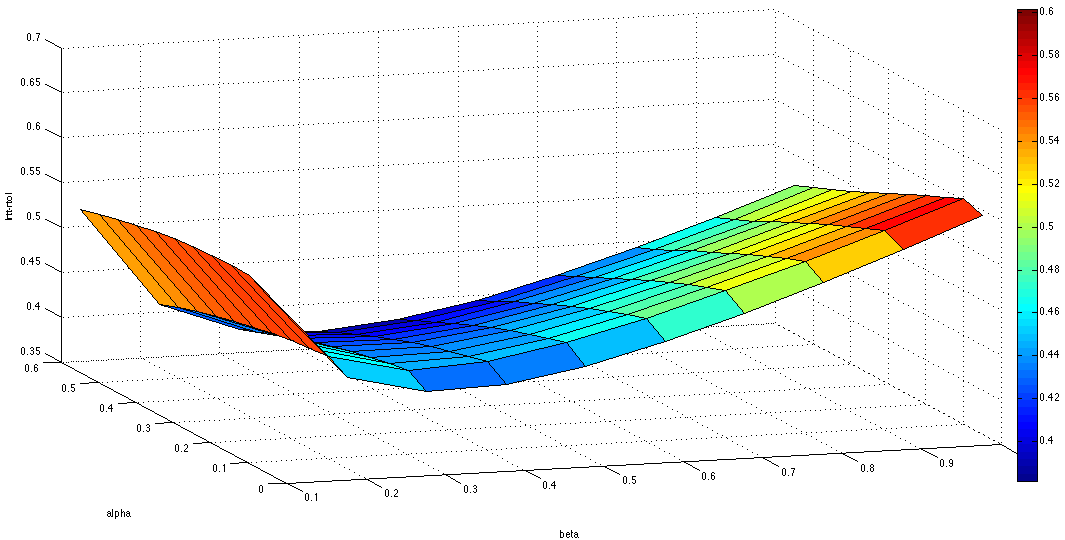
\includegraphics[width=17cm]{alphaBetaCorteCostado.png}
\caption{$|$RTT-RTO$|$ en función de $\alpha$ y $\beta$}
\end{center}
\end{figure}

\begin{figure}[H]
\begin{center}
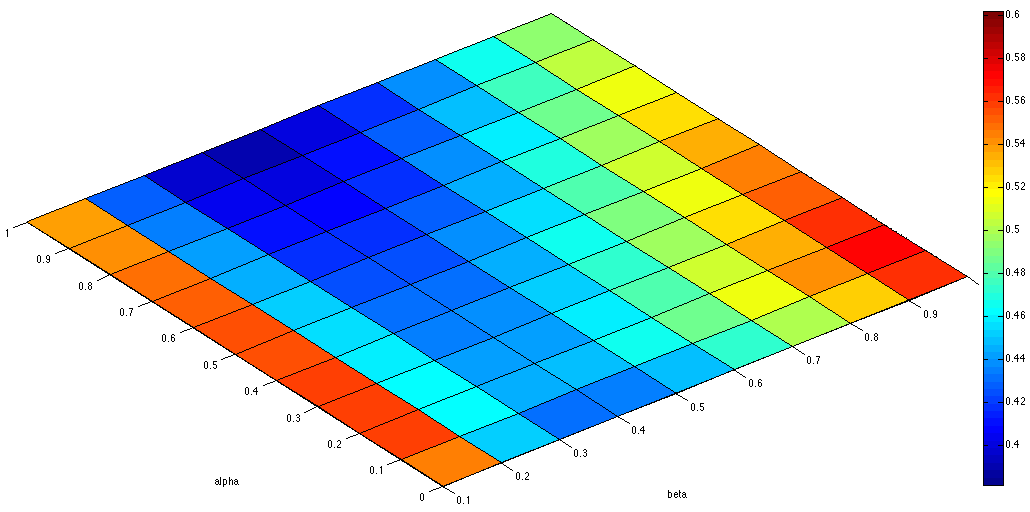
\includegraphics[width=17cm]{alpha-beta-dif-sinCeroB.png}
\caption{$|$RTT-RTO$|$ en función de $\alpha$ y $\beta$}
\end{center}
\end{figure}

A partir de los gráficos anteriores, podemos observar que la mayor diferencia entre los RTT y RTO se da para un valor chico de $\beta$ (0.1) sin importar el valor de $\alpha$ como también para un valor grande de $\beta$ (0.9) combinado con un valor chico a mediano de $\alpha$ (entre 0 y 0.6).
Por otro lado, podemos observar que la diferencia entre los RTT y RTO es menor cuando $\alpha$ ronda valores altos (entre 0.7 y 1) con un $\beta$ entre 0.3 y 0.5.
Por último, notamos que el menor valor de $|$RTT-RTO$|$ se da con $\alpha$ $\in$ [0.9,1] y $\beta$ $\in$ [0.4,0.5].

Dado que con $\beta$ = 0 $|RTT-RTO|$ es muy grande (del orden de 1.9) impidiendo una comparación significativa de los demás valores, decidimos no mostrar los resultados obtenidos para dicha configuración.

\newpage
\subsection{$|$RTT-RTO$|$ en función de $\alpha$ y $\beta$ para un delay fijo}

Por otra parte, nos pareció interesante evaluar el $|$RTT-RTO$|$ en función de $\alpha$ y $\beta$ para un delay fijo. 

Las pruebas realizadas fueron sobre una conexión donde se enviaron 100 paquetes de datos(sin tener en cuenta retransmisiones), y son  las siguientes:

\subsubsection{$|$RTT-RTO$|$ en función de $\alpha$ y $\beta$ con delay en los primeros 50 paquetes}
En primer lugar, decidimos experimentar los $|$RTT-RTO$|$ en función de $\alpha$ y $\beta$ con 0.8 segundos de delay en los primeros 50 paquetes enviados por el cliente.

\begin{figure}[H]
\begin{center}
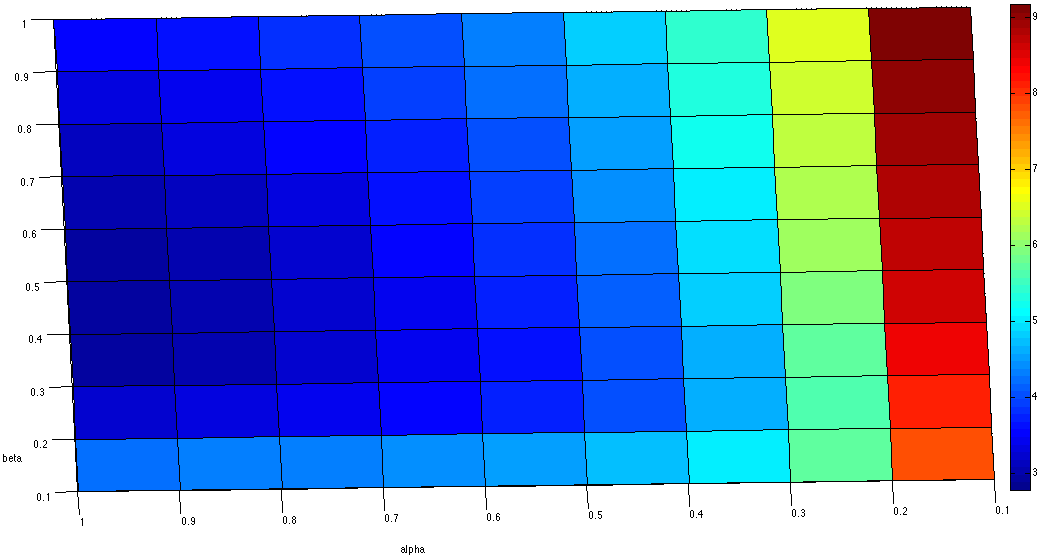
\includegraphics[width=17cm]{delay-50F.png}
\caption{$|$RTT-RTO$|$ en función de $\alpha$ y $\beta$ con delay en los primeros 50 paquetes.}
\end{center}
\end{figure}

Podemos observar que la mayor diferencia entre los RTT y RTO se da para un valor chico de $\alpha$ (0.1) sin importar el valor de $\beta$.
Por otro lado, podemos observar que la diferencia entre los RTT y RTO es menor cuando $\alpha$ ronda valores altos (entre 0.8 y 1) con un $\beta$ entre 0.3 y 0.6.
Por último, notamos que el menor valor de $|$RTT-RTO$|$ se da con $\alpha$ $\in$ [0.9,1] y $\beta$ $\in$ [0.4,0.6].

\subsubsection{$|$RTT-RTO$|$ en función de $\alpha$ y $\beta$ con delay en los últimos 50 paquetes}
Luego, realizamos la misma experimentación de los $|$RTT-RTO$|$ en función de $\alpha$ y $\beta$ con 0.8 segundos de delay pero en los últimos 50 paquetes enviados por el cliente.

%\begin{figure}[H]
%\begin{center}
%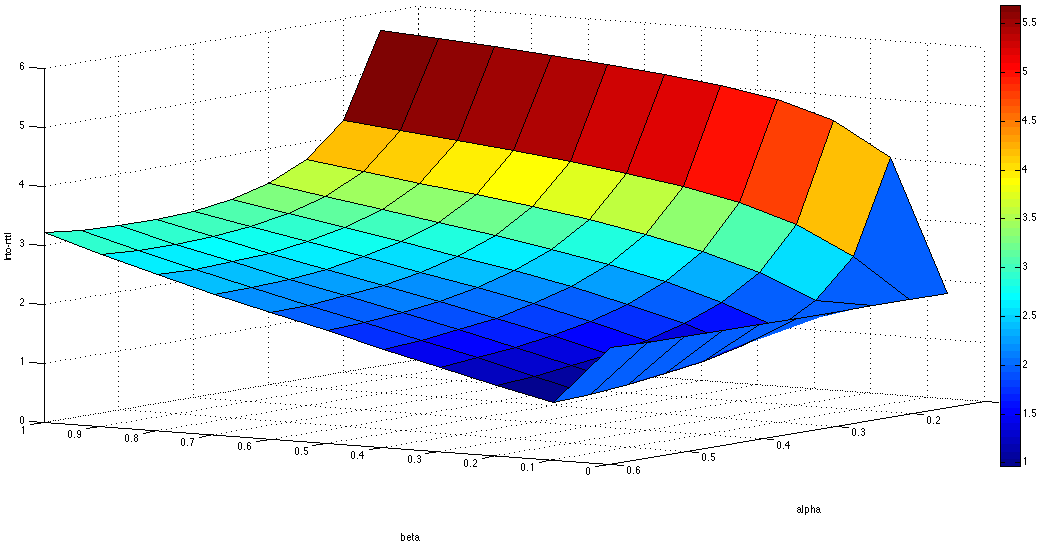
\includegraphics[width=17cm]{delay-50L.png}
%\caption{$|$RTT-RTO$|$ en función de $\alpha$ y $\beta$ con delay en los últimos 50 paquetes.}
%\end{center}
%\end{figure}

\begin{figure}[H]
\begin{center}
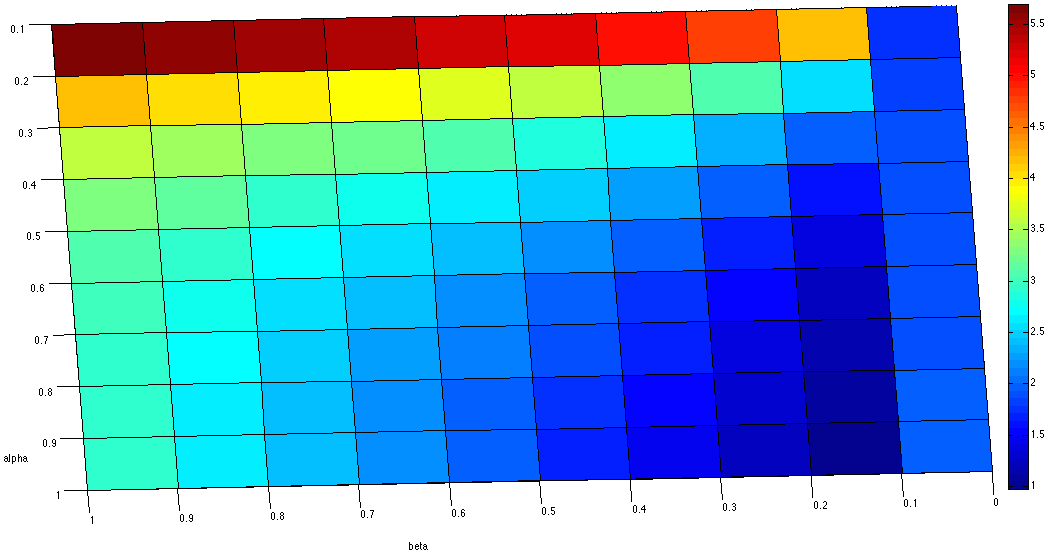
\includegraphics[width=17cm]{delay-50L-costado.png}
\caption{$|$RTT-RTO$|$ en función de $\alpha$ y $\beta$ con delay en los últimos 50 paquetes.}
\end{center}
\end{figure}

Podemos observar que la mayor diferencia entre los RTT y RTO se da para un valor chico de $\alpha$ entre (0.1 y 0.2) y $\beta$ entre (0.1 y 1).
Por otro lado, podemos observar que la diferencia entre los RTT y RTO es menor cuando $\alpha$ ronda valores altos en combinación con $\beta$ rondando valores chicos.
Por último, notamos que el menor valor de $|$RTT-RTO$|$ se da con $\alpha$ $\in$ [0.8,1] y $\beta$ $\in$ [0.1,0.2].

\subsubsection{$|$RTT-RTO$|$ en función de $\alpha$ y $\beta$ con delay en los primeros y últimos 30 paquetes}
Por otro lado, evaluamos las variaciones producidas al medir los $|$RTT-RTO$|$ en función de $\alpha$ y $\beta$ con 0.8 segundos de delay en los primeros y últimos 30 paquetes enviados por el cliente.

\begin{figure}[H]
\begin{center}
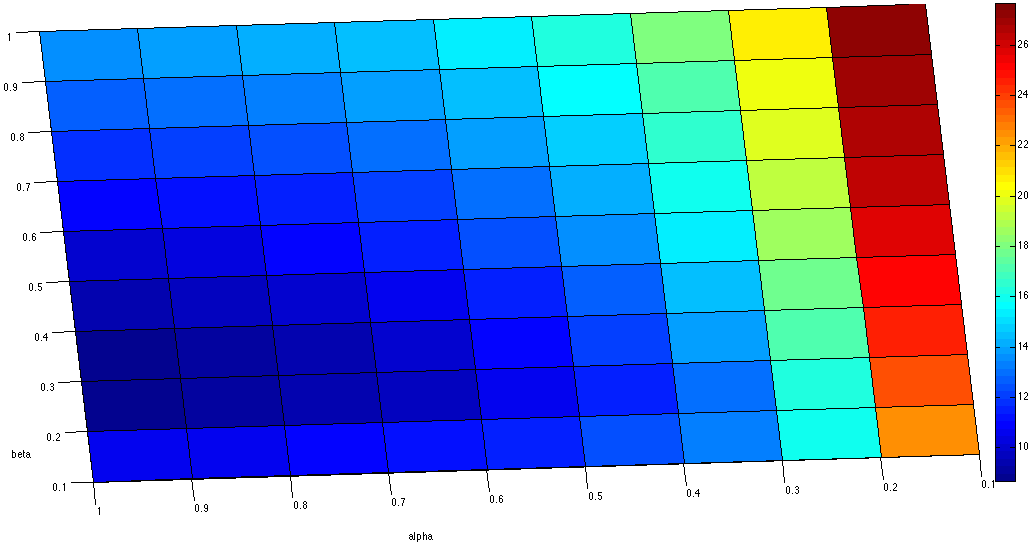
\includegraphics[width=17cm]{delay-30F30L-costado.png}
\caption{$|$RTT-RTO$|$ en función de $\alpha$ y $\beta$ con delay en los primeros y últimos 30 paquetes.}
\end{center}
\end{figure}

Podemos observar que la mayor diferencia entre los RTT y RTO se da para un valor chico de $\alpha$ entre (0.1 y 0.2) sin importar el valor de $\beta$.
Por otro lado, podemos observar que la diferencia entre los RTT y RTO es menor cuando $\alpha$ ronda valores altos en combinación con $\beta$ rondando valores chicos.
Por último, notamos que el menor valor de $|$RTT-RTO$|$ se da con $\alpha$ $\in$ [0.9,1] y $\beta$ $\in$ [0.2,0.4].


\subsubsection{$|$RTT-RTO$|$ en función de $\alpha$ y $\beta$ con delay en los 30 paquetes intermedios}
Posteriormente, medimos los $|$RTT-RTO$|$ en función de $\alpha$ y $\beta$ con 0.8 segundos de delay en los 30 paquetes intermedios enviados por el cliente.

\begin{figure}[H]
\begin{center}
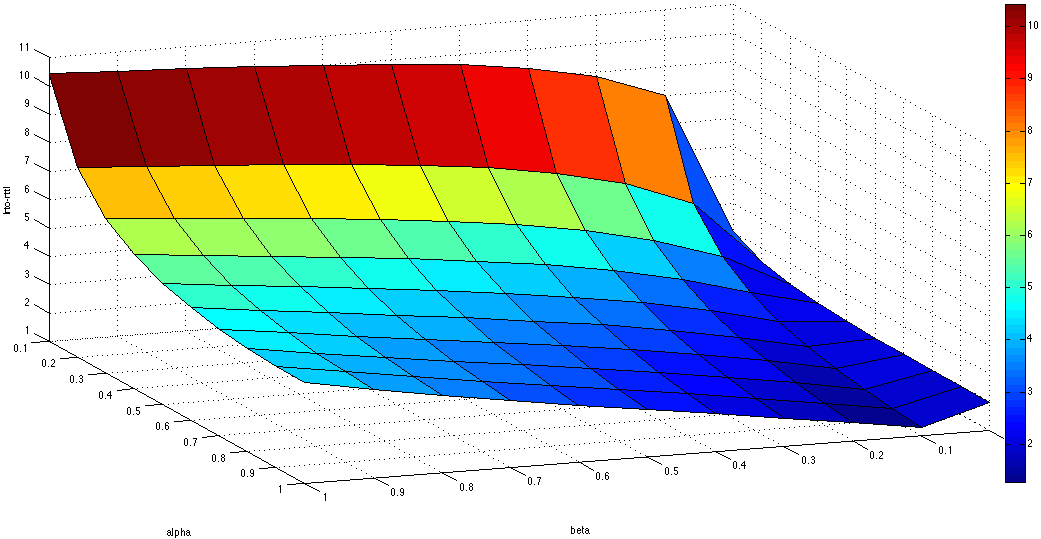
\includegraphics[width=17cm]{delay-30I.png}
\caption{$|$RTT-RTO$|$ en función de $\alpha$ y $\beta$ con delay en los 30 paquetes intermedios.}
\end{center}
\end{figure}

%\begin{figure}[H]
%\begin{center}
%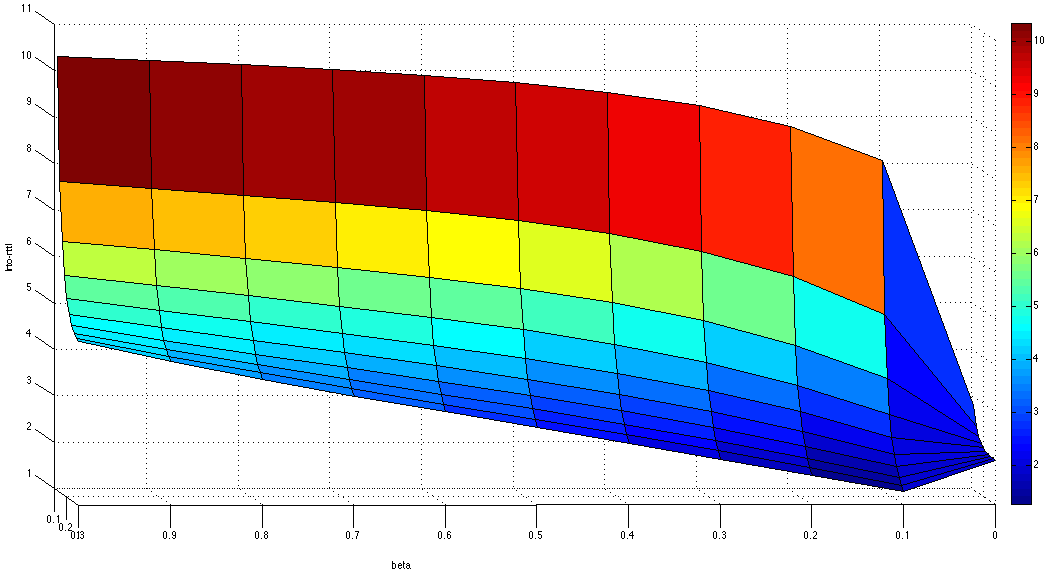
\includegraphics[width=17cm]{delay-30I-costado.png}
%\caption{$|$RTT-RTO$|$ en función de $\alpha$ y $\beta$ con delay en los 30 paquetes intermedios.}
%\end{center}
%\end{figure}
Podemos observar que la mayor diferencia entre los RTT y RTO se da para un valor chico de $\alpha$ (0.1) sin importar el valor de $\beta$.
Por otro lado, podemos observar que la diferencia entre los RTT y RTO es menor cuando $\alpha$ ronda valores altos en combinación con $\beta$ rondando valores chicos.
Por último, notamos que el menor valor de $|$RTT-RTO$|$ se da con $\alpha$ $\in$ [0.9,1] y $\beta$ $\in$ [0.1,0.2].


\subsubsection{$|$RTT-RTO$|$ en función de $\alpha$ y $\beta$ con delay en los primeros y últimos 30 paquetes con delay de 2 segundos}
Por último, decidimos variar el delay llevándolo a 2 segundos, y experimentar los $|$RTT-RTO$|$ en función de $\alpha$ y $\beta$ en los primeros y últimos 30 paquetes enviados por el cliente.

\begin{figure}[H]
\begin{center}
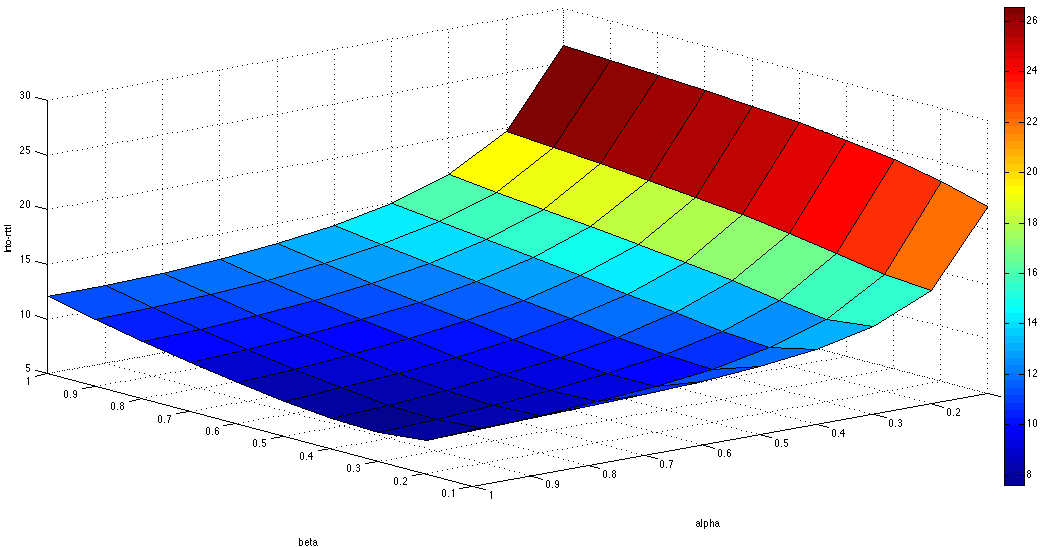
\includegraphics[width=17cm]{delay-30F30L-2seg.png}
\caption{$|$RTT-RTO$|$ en función de $\alpha$ y $\beta$ con delay en los primeros y últimos 30 paquetes.}
\end{center}
\end{figure}

%\begin{figure}[H]
%\begin{center}
%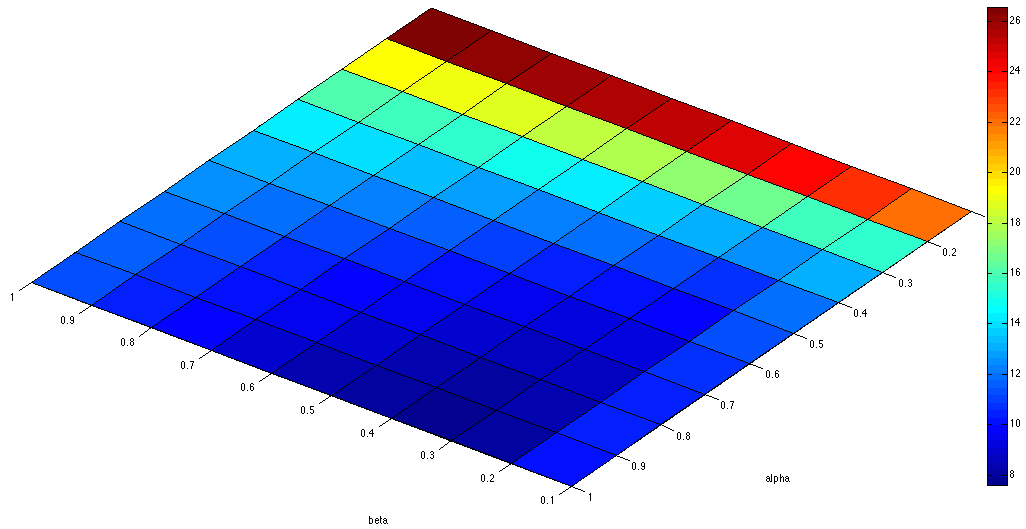
\includegraphics[width=17cm]{delay-30F30L-2seg-costado.png}
%\caption{$|$RTT-RTO$|$ en función de $\alpha$ y $\beta$ con delay en los primeros y últimos 30 paquetes.}
%\end{center}
%\end{figure}

Podemos observar que la mayor diferencia entre los RTT y RTO se da para un valor chico de $\alpha$ (0.1) sin importar el valor de $\beta$.
Por otro lado, podemos observar que la diferencia entre los RTT y RTO es menor cuando $\alpha$ ronda valores altos en combinación con $\beta$ rondando valores chicos.
Por último, notamos que el menor valor de $|$RTT-RTO$|$ se da con $\alpha$ $\in$ [0.9,1] y $\beta$ $\in$ [0.2,0.3].
Estos resultados son similares a los realizados anteriormente con menor delay. Por lo que un incremento mayor del delay en la transmisión del paquete no afecta los resultados.

\newpage
\subsection{Cantidad de retransmisiones en función de $\alpha$ y $\beta$}
Por otro lado, nos pareció interesante mostrar la cantidad de retransmisiones realizadas en el protocolo en función de $\alpha$ y $\beta$. Para ello, alteramos la probabilidad de pérdida de paquetes (esto es, de no envío de los mismos). 

Los resultados de dichas experimentaciones fueron los siguientes:
\begin{figure}[H]
\begin{center}
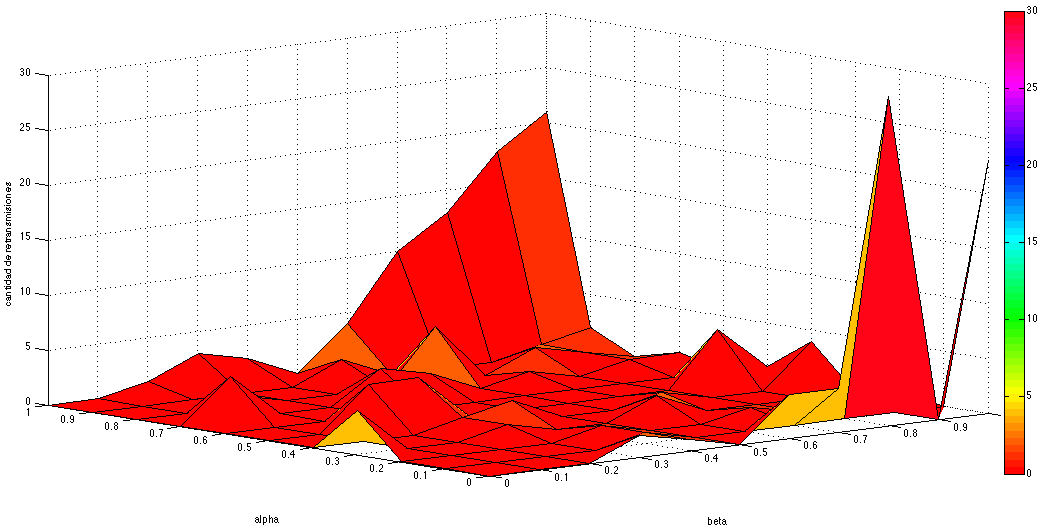
\includegraphics[width=17cm]{alphaBetaRetransmision0,2.png}
\caption{Cantidad de retransmisiones en función de $\alpha$ y $\beta$ con pérdida de 20\% de paquetes.}
\end{center}
\end{figure}

\begin{figure}[H]
\begin{center}
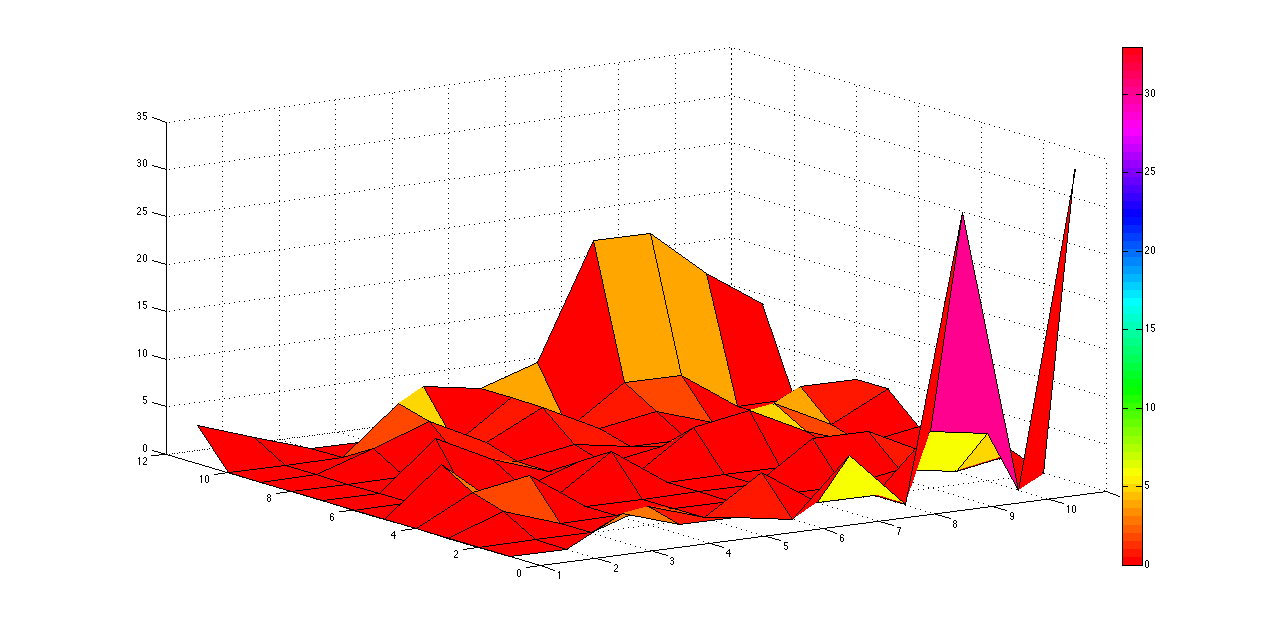
\includegraphics[width=17cm]{alphaBetaRetransmision0,5.png}
\caption{Cantidad de retransmisiones en función de $\alpha$ y $\beta$ con pérdida de 50\% de paquetes.}
\end{center}
\end{figure}

Se puede observar que con pérdidas de paquetes del 20\% y 50\%, no se pueden determinar patrones claros en la cantidad de retransmisiones en función de $\alpha$ y $\beta$. Luego, podemos determinar que dichos valores no afectan la cantidad de retransmisiones de paquetes.

Por otro lado, nos pareció interesante estudiar la cantidad de retransmisiones en casos con delay:

\begin{figure}[H]
\begin{center}
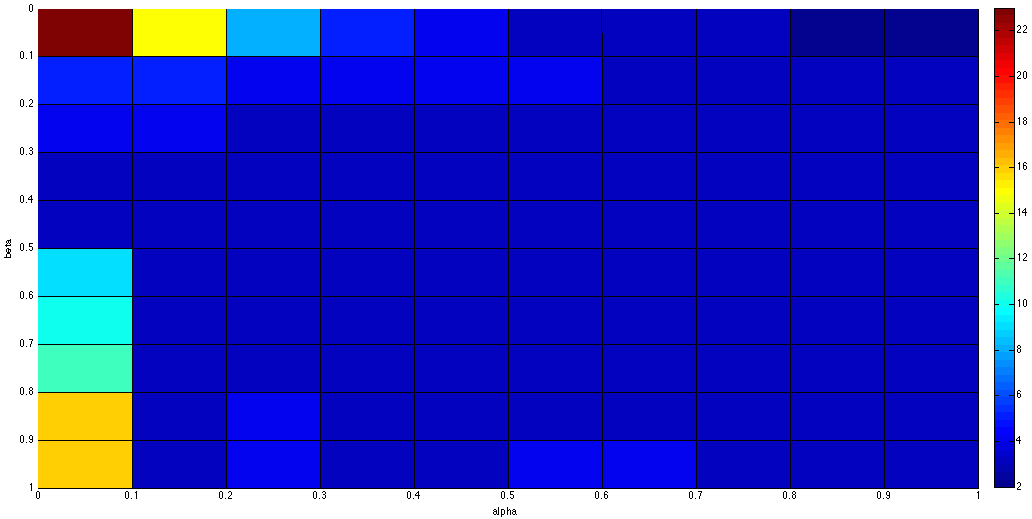
\includegraphics[width=17cm]{delay-30F30L-ret.png}
\caption{Cantidad de retransmisiones en función de $\alpha$ y $\beta$ con delay en los 30 paquetes intermedios.}
\end{center}
\end{figure}

\begin{figure}[H]
\begin{center}
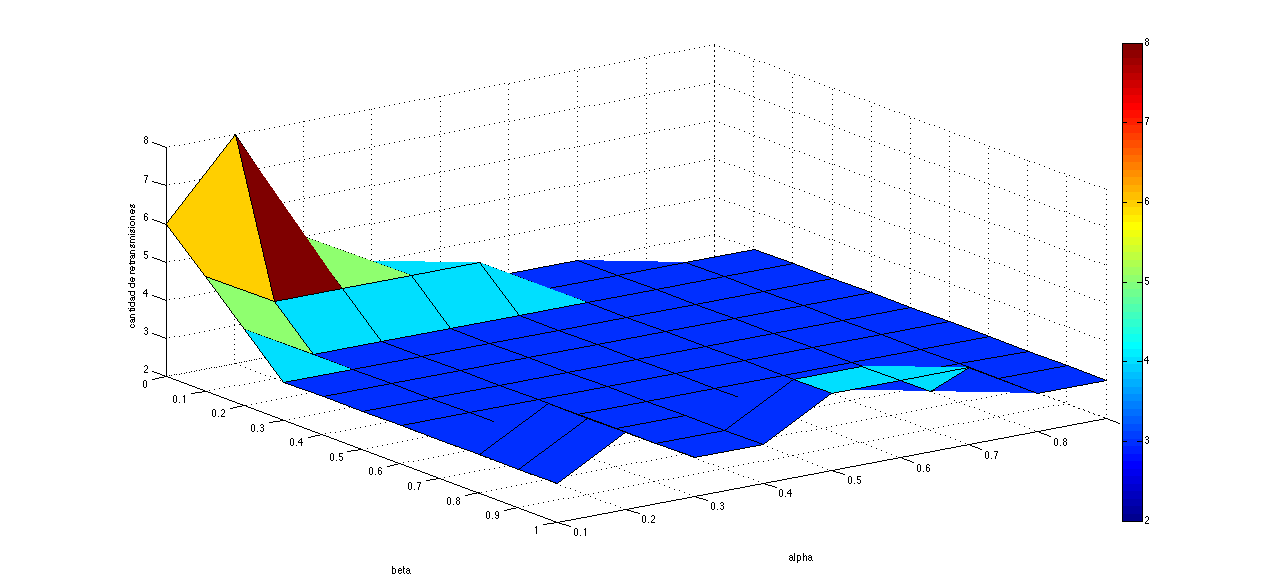
\includegraphics[width=17cm]{delay-30F30L-ret-costado.png}
\caption{Cantidad de retransmisiones en función de $\alpha$ y $\beta$ con delay en los 30 paquetes intermedios.}
\end{center}
\end{figure}


\begin{figure}[H]
\begin{center}
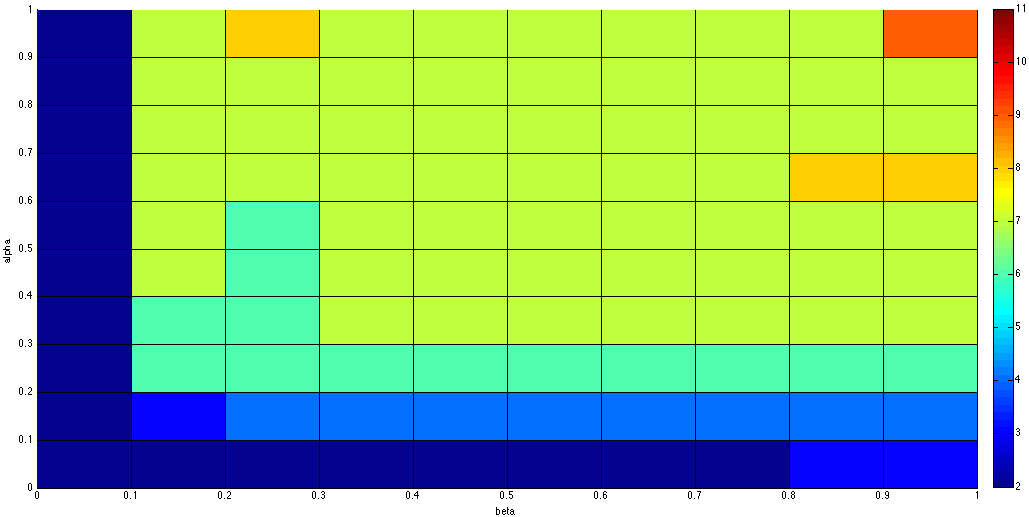
\includegraphics[width=17cm]{delay-30I-ret-costado.png}
\caption{Cantidad de retransmisiones en función de $\alpha$ y $\beta$ con delay en los primeros y últimos 30 paquetes.}
\end{center}
\end{figure}

\begin{figure}[H]
\begin{center}
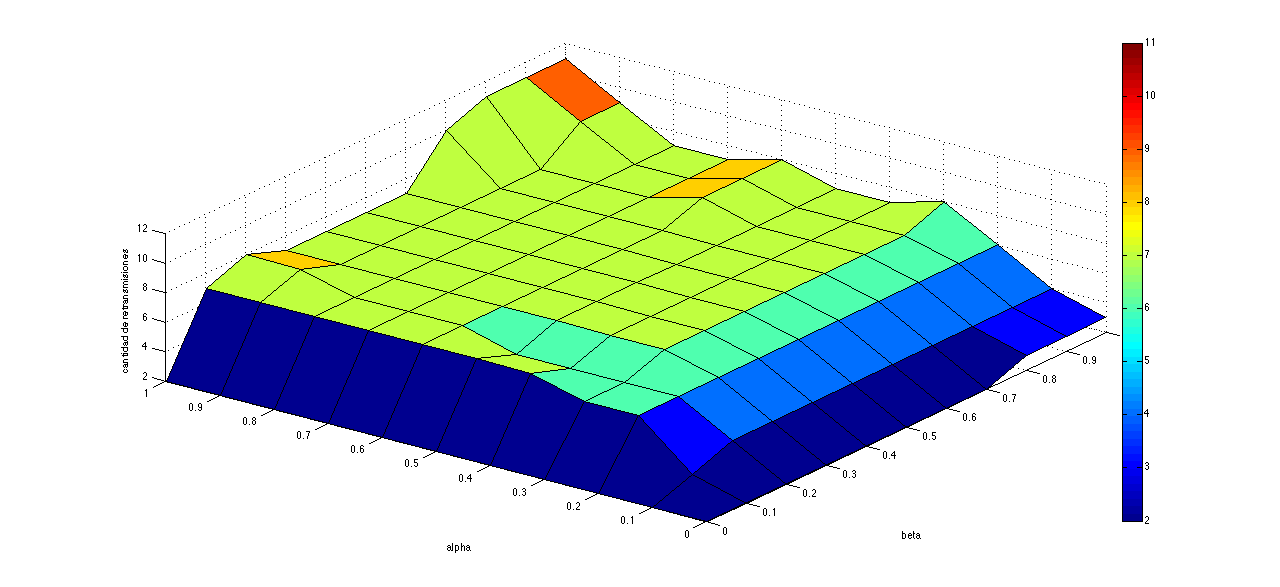
\includegraphics[width=17cm]{delay-30I-ret.png}
\caption{Cantidad de retransmisiones en función de $\alpha$ y $\beta$ con delay en los primeros y últimos 30 paquetes.}
\end{center}
\end{figure}


\begin{figure}[H]
\begin{center}
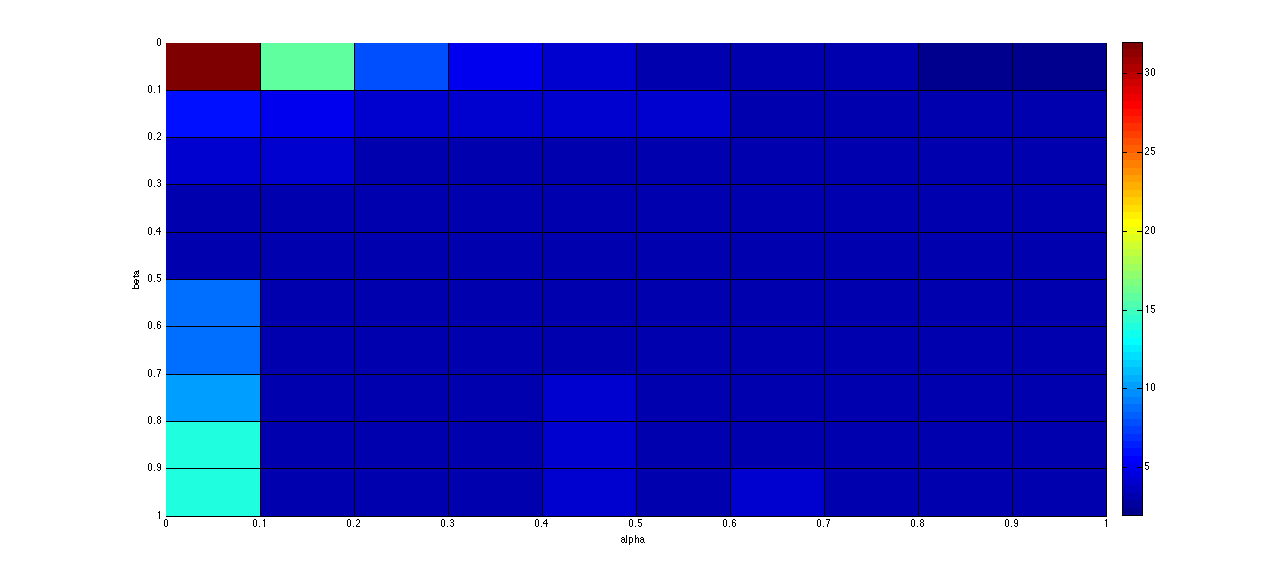
\includegraphics[width=17cm]{delay-50F-ret-costado.png}
\caption{Cantidad de retransmisiones en función de $\alpha$ y $\beta$ con delay en los últimos 50 paquetes.}
\end{center}
\end{figure}

\begin{figure}[H]
\begin{center}
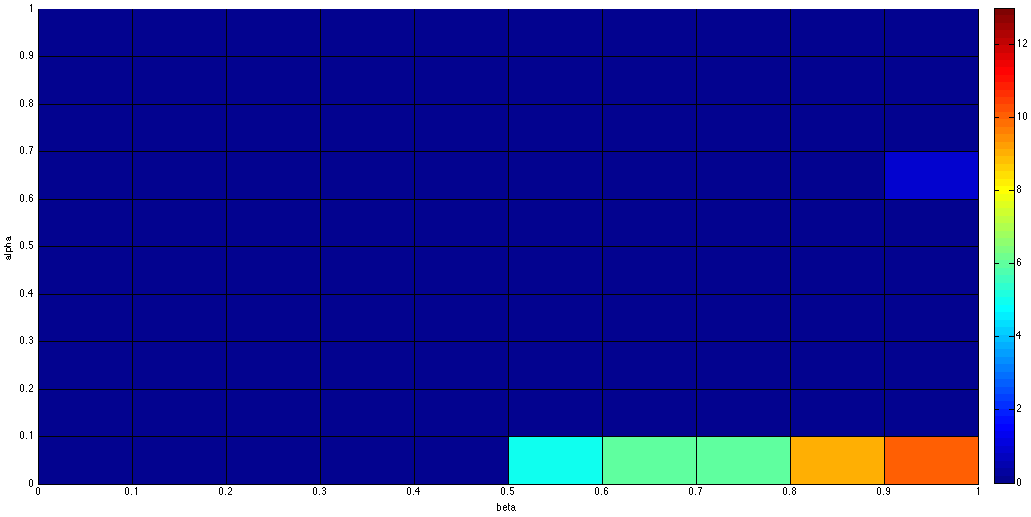
\includegraphics[width=17cm]{delay-50L-ret-costado.png}
\caption{Cantidad de retransmisiones en función de $\alpha$ y $\beta$ con delay en los primeros 50 paquetes.}
\end{center}
\end{figure}

%\begin{figure}[H]
%\begin{center}
%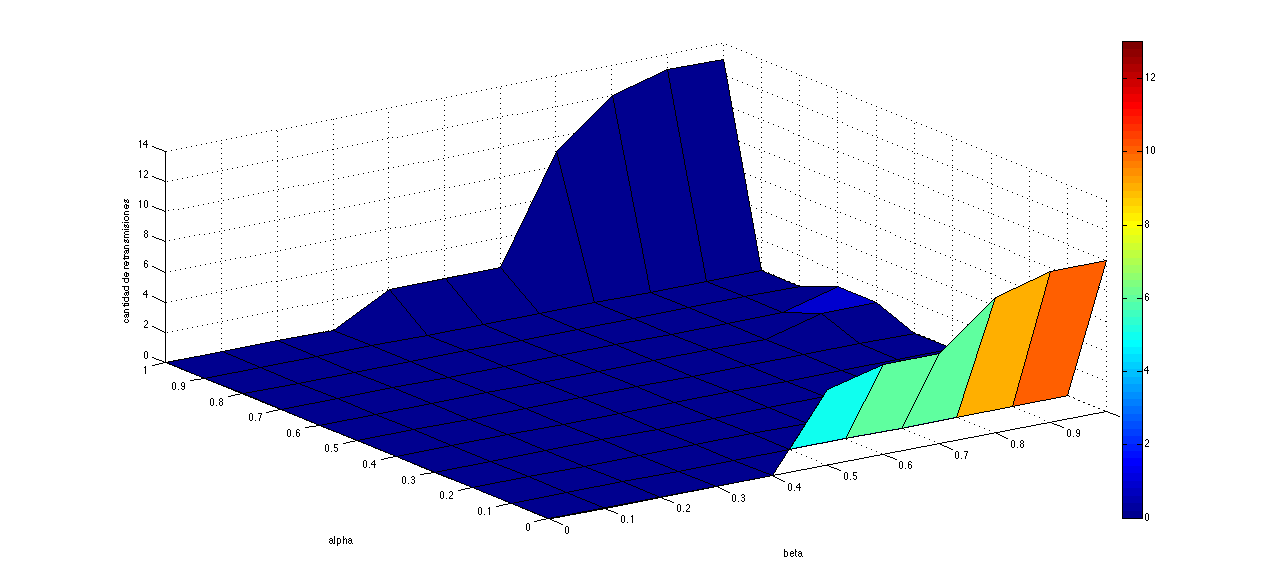
\includegraphics[width=17cm]{delay-50L-ret.png}
%\caption{Cantidad de retransmisiones en función de $\alpha$ y $\beta$ con delay en los primeros 50 paquetes.}
%\end{center}
%\end{figure}

\newpage
\section{Análisis}
En los gráficos de la sección anterior, pudimos observar que los mejores valores que aproximan el RTO del RTT son $ 0.8 \leq \alpha \leq 1$ y $ 0.3 \leq  \beta \leq 0.6$. Estos valores fueron los obtenidos en los test realizados agregando delay para simular congestión en la red.
Sin embargo, en los experimentos realizados para medir la cantidad de retransmisiones, vimos que los mejores valores obtenidos para que ésta sea mínima es de $ 0.1 \leq \alpha \leq 0.3$ y $ 0.1 \leq  \beta \leq 0.3$.

\newpage
\section{Conclusiones}
A partir de la experimentación realizada, pudimos ver qué valores de $\alpha$ y $\beta$ mejor aproximan al RTT del RTO y minimizan la cantidad de retransmisiones de los paquetes.
Por otro lado, hallamos que dichos valores de $\alpha$ y $\beta$ son cercanos a los recomendados en el RFC-6298, por lo que concluimos que los mismos podrían haber sido elegidos a partir de las variables que se debieron analizar en el transcurso del trabajo práctico.

\section{Referencias}
\begin{itemize}
\item PETERSON, DAVIE ; Computer Networks, 5th edition, Wiley

\item{RFC6298: Computing TCP's Retransmission Timer}

\item{STEVENS W., RICHARD; TCP/IP Illustrated, Volume 1: The Protocols Addison-Wesley (1993)}

\end{itemize}
\end{document}
